\subsection{Long Term Evolution (LTE)}
\label{sub:LTE}
	\subsubsection{Arquitectura de la red LTE}
	\label{ssub:arquiLTE}
		\begin{figure}[htp]
			\centering
			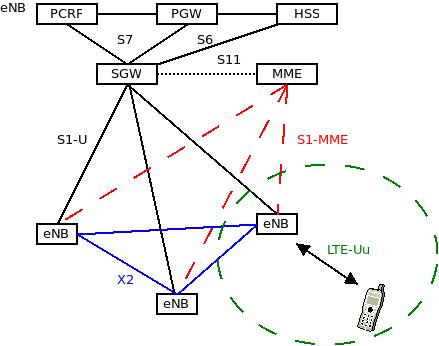
\includegraphics[width=0.7\textwidth]{Imagen/diaLTE.jpg}
			\caption{Arquitectura de la red LTE}
		\end{figure}
		\begin{itemize}
			\item e-NodeB Se ocupa de la gestión de los recursos radio, control de interferencias, compresión de cabeceras IP, cifrado y proteccion de la integridad de datos de usuario, selección del MME y el encaminamiento hacia el S-GW.
			\item Entidades Evolved Packet Core (EPC)
			\begin{itemize}
				\item Mobility Management Entity (MME) Se ocupa del control de acceso, gestión del área de tracking y paging, itinerancia, autentificación y gestiona la selección tanto de S-GW como de P-GW.
				\item Serving Gateway (S-GW) Es la entidad que se ocupa del encaminamiento de paquetes, los niveles de QoS. Cada móvil solo podrá estar conectado a una única S-GW al mismo tiempo.
				\item Packet Data Network Gateway (P-GW) Se encarga del filtrado de pauetes, del marcado del QoS en el nivel del transporte, de la adjudicación de una dirección IP al móvil y del anclaje del terminal para la movilidad.
			\end{itemize}
			\item Home Suscriber Server (HSS). Se trata del antiguo HLR.
			\item Equipment Identity Register (EIR). La misma lista negra que en sistemas anteriores
			\item Policy \& Charging Rules Function (PCRF) se encarga de la facturación por flujo.
		\end{itemize}
	% subsubsection arquiLTE (end)
	\subsubsection{Características Generales de LTE}
	\label{ssub:caracLTE}
		\begin{itemize}
			\item Movilidad: Es un sistema optimizado para bajas velocidades, 0 a 15 km/h, pero que permite ofrecer un alto rendimiento hasta velocidades considerables, 15 a 120km/h. El límite producido por el efecto dopler se encuentra en los 350km/h.
			\item Cobertura: Para obtener los mejores resultados se pueden llegar a crear celdas de 5km de radio. Rebajando la calidad de la cobertura se pueden llegar a obtener celdas de 30km de radio.
			\item Capacidad de celda: El requisito es que se pueda dar servicio, al menos, a 200 usuarios activos por celda.
			\item Modulación:
			\begin{itemize}
				\item En subida se utiliza SC-FDMA, otorgando los recursos al ususario con las mejores condiciones instantaneas.
				\item En bajada se utiliza OFDMA, por su robustez, flexibilidad y todas las técnicas avanzadas de procesamiento.
			\end{itemize}
			\item Constelaciones:
			\begin{itemize}
				\item En subida se utilizan QPSK, 16QAM y en ciertas ocasiones se puede llegar a 64QAM. El canal PRACH utiliza otra modulación.
				\item En bajada se utilizan QPSK, 16QAM y 64QAM para datos y BPSK y QPSK  para canales de control.
			\end{itemize}
			\item Baja latencia, es decir, los tiempos de set-up y los retardos de retransmisión son cortos.
			\item Codificación: Basada en turbo coding o Tail Biting Convoltional Coding (TBCC). La modulación y el esquema de codificación son variables.
			\item Duplexación, se permite tanto en frecuencia como en tiempo. Así los terminales simples pueden ser compatibles.
			\item No hay macrodiversidad, se produce traspaso duro debido al OFDM.
			\item Arquitectura de protocolos simple basada en canales compartidos dentro de un único dominio, el de paquetes, con vozIP.
			\item Arquitectura de red simple: Solo hay eNodesB conectados mediante pocas interfaces, X2 y S1.
		\end{itemize}
	% subsubsection caracLTE (end)
	\subsubsection{Canales LTE}
	\label{ssub:canalesLTE}
		\begin{itemize}
			\item Canales Físicos:
			\begin{itemize}			
				\item Physical Random Access Channel (PRACH)
				\item Physical Uplink Control Channel (PUCCH)
				\item Physical Uplink Shared Channel (PUSCH)
			\end{itemize}
			\item Señales Físicas:
			\begin{itemize}
				\item Sounding Reference Signal (SRS)
				\item Demodulation Reference Signal (DM-RS)
			\end{itemize}
		\end{itemize}
		\begin{figure}[H]
			\centering
			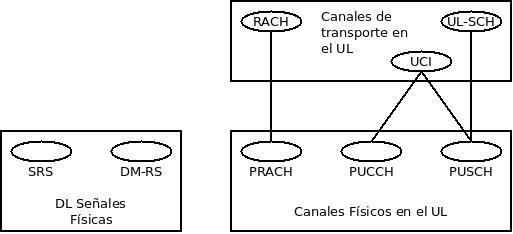
\includegraphics[width=\textwidth]{Imagen/canalesAscendente.jpg}
			\caption{Canales del enlace ascendente}
		\end{figure}
		\begin{itemize}
			\item Physical Broadcast Channel (PBCH)
			\item Physical Downlink Shared Channel (PDSCH)
			\item Physical Control Format Indicator Channel (PCFICH)
			\item Physical Downlink Control Channel (PDCCH)
			\item Physical HARQ Indicator Channel (PHICH)
			\item Physical Multicast Channel (PMCH)
		\end{itemize}
		\begin{figure}[H]
			\centering
			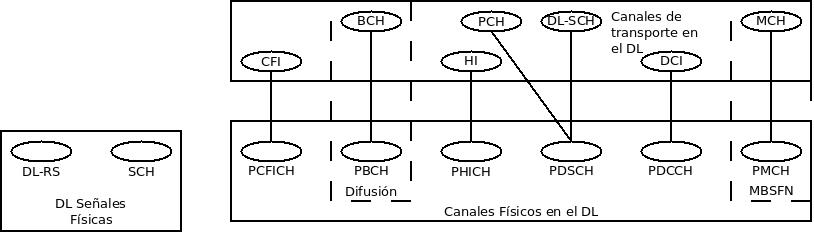
\includegraphics[width=\textwidth]{Imagen/canalesDescendente.jpg}
			\caption{Canales del enlace Descendente}
		\end{figure}
	% subsubsection canalesLTE (end)
% subsection LTE )